\chapter{Wykorzystane technologie}
\label{cha:tech-stack}

\section{Amazon Web Services}
Amazon Web Services (AWS) jest najpopularniejszym dostawcą usług cloudowych na świecie \cite{AWS-what}. 
Swoją pozycję zawdzięcza nieustannemu rozwojowi swoich produktów i wsłuchiwaniu się w potrzeby klientów.
Duże znaczenie ma również fakt, że Amazon.com jest również zbudowany na swojej platformie \cite{AS3}.
Klienci z ponad 190 krajów aktywnie korzystają z rozrastającego się wachlarza 175+ produktów, serwowanych przez centra danych położone na całym świecie \cite{AWS-O}.
AWS innowacje wprowadza już na poziomie hardware'u - projektuje własne wyspecjalizowane komponenty na użytek swoich serwerowni.
Jednym z najnowszych przykładów jest Nitro Card, 
który redefiniuje tradycyjne podejście do wirtualizacji obniżając przy tym koszty, zwiększając wydajność i bezpieczeństwo \cite{AWS-Nitro}.

\subsection{EC2}
Podstawowy produkt AWS zapewniający nam wirtualne lub {\em bare metal} instancje serwerów. 
Przychodzący i wychodzący ruch internetowy kontrolujemy przy pomocy wirtualnego firewalla - Security Group.
Poprzez mechanizm EC2 Auto Scaling możemy zdefiniować zasady ich skalowania horyzontalnego do aktualnych potrzeb.
Oferowane typy instancji różnią się dedykowanym przeznaczeniem \cite{AWS-Nitro}:

\begin{itemize}
    \item
    \textbf{M5: General Purpose}\\
    {\em Monolityczne aplikacje biznesowe}
    
    \item
    \textbf{T3: General Purpose - Burstable}\\
    {\em Mikroserwisy, interaktywne aplikacje wymagające niskiej latencji}

    \item
    \textbf{C5: Compute Optimized}\\
    {\em Aplikacje wymagające wysokiej wydajności}

    \item
    \textbf{P3dn: Machine Learning}\\
    {\em Wysoko wydajne uczenie maszynowe}

    \item
    i wiele innych
\end{itemize} 

Obraz możemy wybrać z bazowego zestawu Linux'ów i Windows'ów lub zasięgnąć AWS Marketplace, gdzie zamieszczane są obrazy budowane przez szerszą społeczność.

\subsection{DynamoDB}
Baza danych NoSQL w pełni zarządzana przez AWS. 
Zaimplementowana z myślą o wysokiej wydajności niezależnie od aktualnej skali, operacje realizowane są w jedno cyfrowej ilości milisekund.
Od użytkownika wymaga się jedynie zdefiniować strukturę tabeli. Utrzymanie i skalowanie bierze na siebie AWS \cite{AWS-O}.

\subsection{S3}
Wszechstronny serwis do przechowywania plików, używany często przez inne produkty AWS {\em (np. DynamoDB przechowuje backup'y na S3)}. 
Jednym z popularniejszych przypadków użycia jest hostowanie na S3 aplikacji webowych. 
Jak każdy z podstawowych serwisów zarządzanych przed AWS, S3 jest przygotowane na każdą skalę, zachowując przy tym wydajność i bezpieczeństwo \cite{AWS-O}.

\subsection{Route53}
Bogaty, zintegrowany z platformą serwis DNS. Najczęściej używany by nakierować ruch na instancje EC2. 
Udostępniona jest również opcja zakupu domeny bezpośrednio w konsoli webowej AWS co przyspiesza gotowość jej użycia.

\subsection{CloudFormation} \label{cloudFormation}
Obowiązkowe narzędzie przy pracy z większą ilością instancji produktów AWS. 
Całą swoją infrastrukturę definiuje się w czytelnym formacie pliku tekstowego {\em yaml} lub {\em json}.
Z tak przygotowanym plikiem przełożenie definicji na świat rzeczywisty jest dosłownie jednym kliknięciem. 
Równie łatwo wykonamy aktualizację lub pozbędziemy się wszystkich utworzonych produktów \cite{AWS-O}.
Taką automatyzację udostępnia również open source'owy odpowiednik tego narzędzia - Terraform.


\section{Docker}

\subsection{Maszyny wirtualne}

Tradycyjne podejście do wirtualizacji skupia się na abstrakcji fizycznego sprzętu. 
Pozwala to na traktowanie jednego hosta jako wiele serwerów. 
Każda wirtualna maszyna zawiera pełną kopię systemu operacyjnego, wszystkie potrzebne narzędzia i pliki docelowej aplikacji, sumując wszystko często otrzymamy dziesiątki GB.
Uruchomienie takich jednostek jest dosyć wolne {\em (kilka minut)} \cite{docker-c}.
    
\subsection{Docker containers}

Docker natomiast jest abstrakcją systemu operacyjnego. Kontenery dockera są odciążone od warstwy OS i zawierają tylko aplikację i potrzebne jej narzędzia.
Każdy kontener działa jako wyizolowany proces. Są dużo lżejsze {\em (zazwyczaj dziesiątki MB)}, 
więc ten host pomieści więcej aplikacji uruchomionych jako kontenery niż jako wirtualne maszyny \cite{docker-c}.

\begin{figure}[h!]
	\begin{center}
		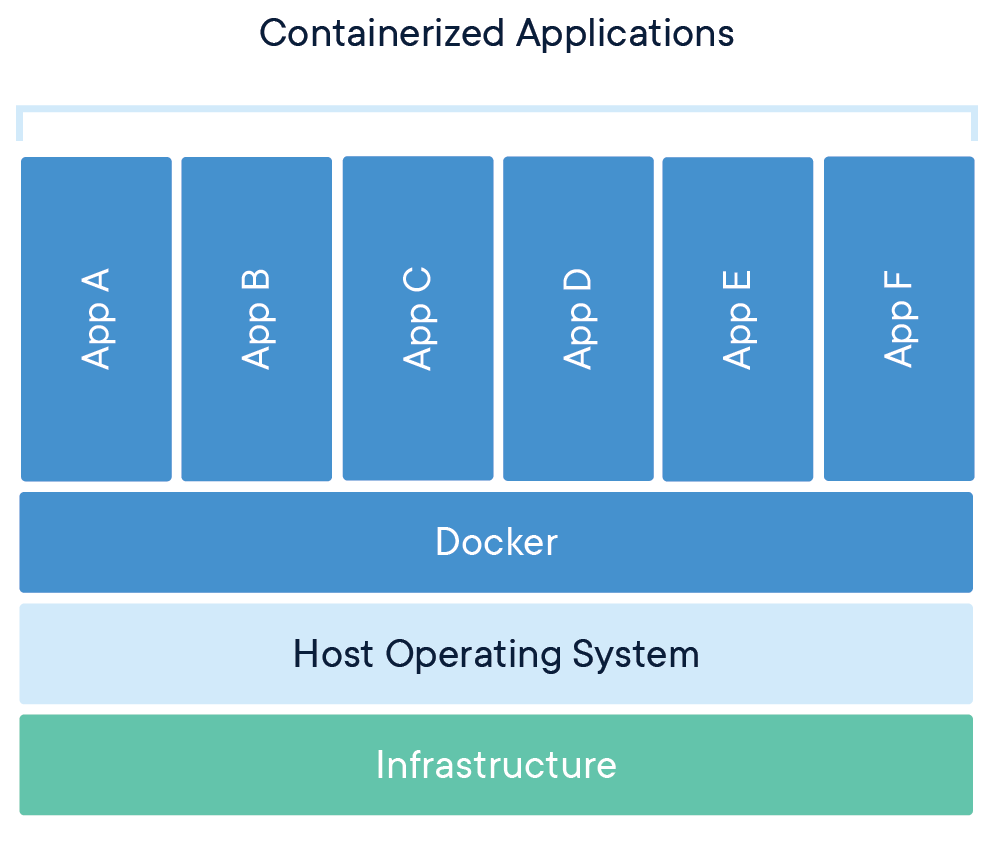
\includegraphics[width=0.45\textwidth]{img/docker-layers}
		\hspace{5mm}
		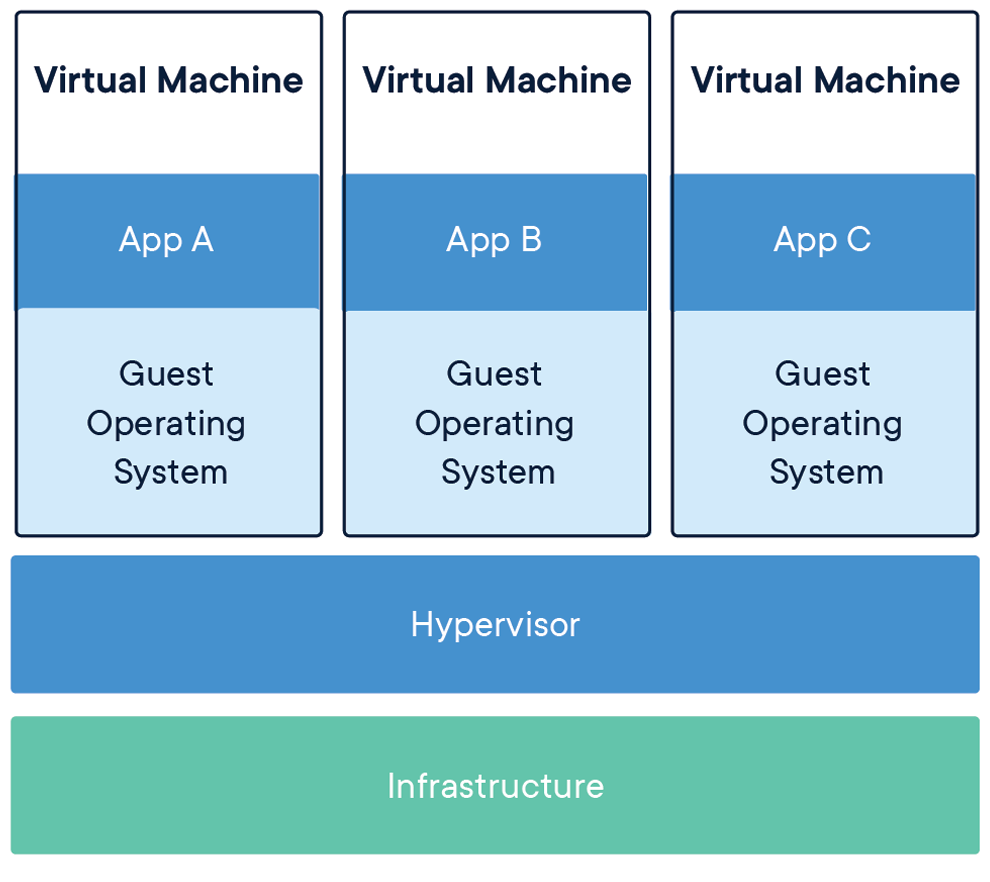
\includegraphics[width=0.45\textwidth]{img/vm-layers}
	\end{center}
	\caption{Docker containers vs VMs \cite{docker-c}.}
	\label{fig:docker-vms}
\end{figure}

\subsection{Docker image}
Jest to plik złożony najczęściej z kilku warstw \cite{docker-doc}. 
Najczęściej wszystkie warstwy oprócz wierchniej są \emph{read-only}, stanowią narzędzia wykorzystywane przez docelową wiechnią aplikację \emph{(np. java sdk)}.
Najwyższa warstwa budowana jest przy pomocy pliku z instrukcją - \emph{\textbf{Dockerfile}}, gdzie dokładamy naszą aplikację.
Przygotowany w ten sposób image jest gotowy do uruchomienia jako kontener. Dużym udogodnieniem dla użytkownika jest globalne publiczne repozytorium docker images - \emph{\textbf{hub.docker.com}}.


\section{Kubernetes}
W zarządzaniu większą ilością produktów AWS stanowiących naszą platformę pomoże nam opisany wcześniej CloudFormation \emph{(\ref{cloudFormation})}. 
Do orkiestracji skonteneryzowanymi aplikacjami posłużymy się wiodącym standardem w tej dziedzinie - Kubernetes.
Projekt jest rezultatem ponad 10-cio letniego doświadczenia Google w tej dziedzinie opublikowanym na zasadach open-source w 2014 roku \cite{k8s-what}.
Rozwiązanie zyskało na nowych pomysłach społeczności i adaptacji przez wszystkich wiodących dostawców usług chmurowych.
Istnieje również możliwość zastosowania Kubernetes we własnej serwerowni, 
co oznacza duży krok w kierunku jednolitego środowiska niezależnie od sposobu hostowania systemu naszej aplikacji.
Całą strukturę kontenerów jak również i wszystkie inne potrzebne zasoby definiujemy w plikach tekstowych {\em yaml} lub {\em json}.

\subsection{Podstawowe funkcje Kubernetes}

\begin{itemize}
    \item
    \textbf{Service discovery \& load balancing}\\
    Funkcjonalności Kubernetes realizują skonteneryzowane aplikacje systemowe niewidoczne dla użytkownika na porządku dziennym.
    Wśród nich znajdziemy grupę odpowiedzialną za wewnątrz systemowy DNS. Ruch rozkładany jest na ukryte za serwisową domeną instancje aplikacji. 
    
    \item
    \textbf{Storage orchestration}\\
    Automatyczne utworzenie zadanego zasobu pamięci na podstawie definicji tekstowej i dołączenie jej pod wskazany kontener.

    \item
    \textbf{Automatic bin packing}\\
    \label{bin-packing}
    Mając do dyspozycji zestaw nodów (hostów), na których umożliwiamy stawianie kontenerów, Kubernetes sam podejmuje decyzje na temat wdrożenia.
    Dzięki temu nie musimy się martwić o przeciążenie pojedynczego noda.
    Poprzez definicje wymagań \emph{(CPU, RAM)} danego kontenera możemy natomiast dostarczyć wskazówki. 

    \item
    \textbf{Autoscaling, Self-healing, Automated rollouts and rollbacks}\\
    Za pomocą plików tekstowych definiujemy oczekiwaną liczbę instancji naszej aplikacji i jej zasady skalowania horyzontalnego \emph{(wpływ CPU, RAM)}.
    Ponadto możemy określić sygnały \emph{(np. zapytanie http)} w oparciu o które Kubernetes może weryfikować zdolność do pracy danej instancji, a następnie podjąć próby jej restartu.
    W przypadku utracenia całego noda (hosta) utracone tam kontenery zostaną przerzucone na resztę nodów do czasu startu nowego.
    Domyślnie update kontenera \emph{(np. do nowej wersji docker image)} polega wpierw na uruchomieniu jego nowej wersji, a dopiero potem przepięciu ruchu i zabiciu starej.
    Jeśli nowy kontener nie spełni wymagań żywotności, zostanie on wycofany. Taki proces zapewnia 100\% dostępności aplikacji \cite{k8s-what}.
\end{itemize} 

\subsection{Podstawowe pojęcia Kubernetes}

\begin{figure}[!ht]
	\begin{center}
		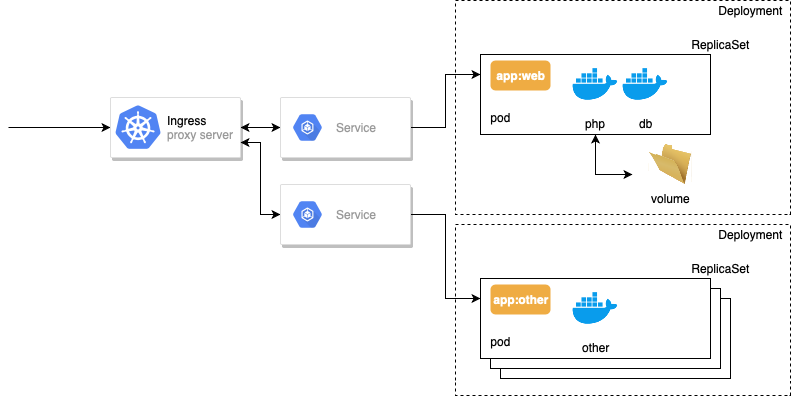
\includegraphics[width=1\textwidth]{img/k8s-objects}
	\end{center}
	\caption{Droga zapytania przez obiekty Kubernetes \cite{k8s-diagram}.}
\end{figure}

\subsubsection{Cluster}
\cw{Node} jest pojedynczą jednostką obliczeniową, może być to fizyczny komputer lub jak w większości przypadków - wirtualna maszyna. 
\cw{Cluster} to grupa \cw{Node}'ów stanowiąca jeden organizm. 
Wdrażając aplikacje nie specyfikujemy na którym \cw{Node}'ie mają stanąć nowe kontenery. Kubernetes nas w tym wręcza \emph{(\ref{bin-packing})}.

\subsubsection{Pod}
\cw{Pod} jest najmniejszym obiektem w świecie Kubernetes jaki możemy wdrożyć. Stanowi pojedynczą instancję aplikacji. 
Najczęśniej zawiera jeden kontener, choć może zawierać ich więcej. 
Kontenery wewnątrz \cw{Pod}'a współdzielą zasoby i unikalny adres IP przydzielony przez orkiestratora \cite{k8s-cpts}.

\subsubsection{ReplicaSet \& Deployment}
Zadaniem \cw{ReplicaSet} jest utrzymanie danej liczby identycznych \cw{Pod}'ów \emph{(instancji danej aplikacji)}.
Jednak w większości przypadków nie będziemy pracować bezpośrednio z \cw{ReplicaSet} tylko z obiektem wyżej w hierarchii - \cw{Deployment}.
Poprzez niego przeskalujemy oczekiwaną liczbę \cw{Pod}'ów i przeporwadzimy \emph{rolling update} \cite{k8s-cpts}.


\subsubsection{Service}
Sposób wystawienia \cw{Pod}'ów aplikacji jako serwis dostępny w sieci. Pozostałe aplikacje odnoszą się do niego korzystając z jego węwnątrz \cw{Cluster}'owej nazwy DNS.
Ruch jest następnie rozkładany pomiędzy cały \cw{ReplicaSet} aplikacji \cite{k8s-cpts}. Do typów \cw{Service} należą: 

\begin{itemize}
    \item
    \textbf{ClusterIP}\\
    Dostęp tylko wewnątrz \cw{Cluster}'a
    
    \item
    \textbf{NodePort}\\
    Dostęp również poza \cw{Cluster}'em poprzez:\\ 
    \emph{<adres IP dowolnego }\cw{Noda}\emph{>:<zdefiniowany port }\cw{Service}\emph{'u>}

    \item
    \textbf{LoadBalancer}\\
    \cw{Service} jest wystawiony poprzez \emph{LoadBalancer} utworzony przez dostawcę platformy chmurowej, na której działa nasz \cw{Cluster}.
\end{itemize} 


\subsubsection{Ingress}
Częstą praktyką jest utworzenie jednego punktu dostępu dla całego \cw{Cluster}’a. 
Wdrażamy wtedy jedną z implementacji \emph{Ingress Controller} (najpopularniejsza to \emph{nginx}, w projekcie używam \emph{Istio} [\ref{istio}]), która stanowi ruter dla pozostałych \cw{Service}’ów. 
\cw{Ingress} to obiekt definiujący rutowanie nadchodzących pakietów (np. na podstawie ścieżki http) \cite{k8s-cpts}.


\section{Istio}
\label{istio}

\begin{figure}[!ht]
	\begin{center}
		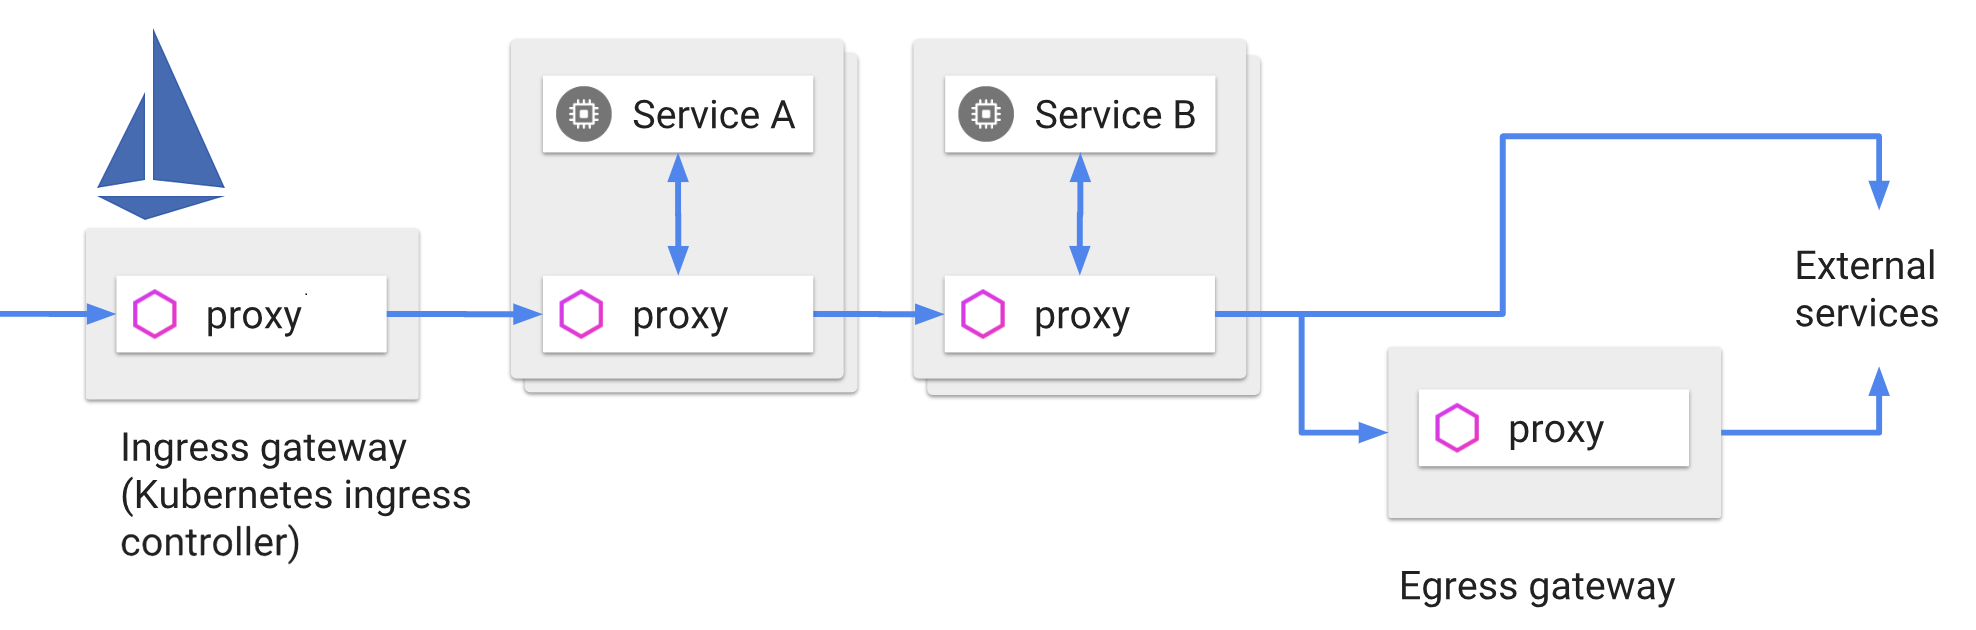
\includegraphics[width=1\textwidth]{img/istio}
	\end{center}
	\caption{Zastosowanie Istio w Kubernetes \cite{istio-traffic}.}
\end{figure}

Wraz z transformacją z monolitycznej aplikacji do sieci mikroserwisów pojawia się wiele nowych problemów związanych z komunikacją pomiędzy nimi.
Kubernetes nie dostarcza żadnego domyślnego rozwiązania, by nie ograniczyć doboru przez użytkownika.
Istio jest jednym z nich, wypuszczone przez \emph{Lyft} i zaadaptowane później przez m.in. \emph{Google} i \emph{Microsoft}. \cite{istio-what}
Istio zapewnia nam:

\begin{itemize}
    \item
    Szczegółową kontrolę nad zachowaniem się ruchu poprzez definicje rutowań, ponowień, failovers i circuit breakers.
    
    \item
    Automatyczne metryki, odkładanie logów i śledzenie ruchu w naszym \cw{Cluster}'rze.

    \item
    Bogate narzędzia do wprowadzenia autentykacji i autoryzacji
    
\end{itemize} 

Włączenie funkcjonalności Istio do \cw{Pod}'a odbywa się poprzez wstrzykniecie pobocznego kontenera, 
który stanowi proxy dla głównego kontenera aplikacji.

\section{Jenkins}

Jenkins jest najpopularniejszym narzędziem do \textbf{CI \& CD} w branży. 
Utrzymywany przez społeczność open source nadąża za zmianami w świecie programowania.
Podstawowe funkcjonalności rozszerza bogaty zbiór pluginów.
Jenkins może być wdrożony na wiele sposobów, w tym projekcie stawiam go jako docker container w środku \cw{Cluster}'a. 

\subsection{Jenkinsfile}
Jest to plik \emph{(groovy syntax)}, w którym definiujemy cały \textbf{\emph{pipeline}} - poszczególne kroki od zaciągnięcia plików źródłowych z SCM do wdrożenia na \cw{Cluster}.
Ponadto przetrzymywany w zdalnym repozytorium stanowi wskaźnik dla Jenkinsa, by dane repozytorium było brane pod uwagę w ramach job'a \emph{"Github Organization"}.

